\documentclass[11pt]{article}
% \documentclass[draft,11pt]{article}
% Package imports and settings {{{1
\usepackage{amsmath}
\usepackage{amssymb}
\usepackage{array}
\usepackage{booktabs}
\usepackage[skip=12pt,labelfont=it,font=small]{caption}
\usepackage{subcaption}
\captionsetup{subrefformat=parens}
\usepackage{float}
\usepackage{fullpage}
\usepackage{graphicx}
\graphicspath{{./figures/}}
\usepackage[version=4]{mhchem}
\usepackage{multirow}
\usepackage{parskip}
\usepackage{setspace}
\usepackage{siunitx}
\usepackage{titlesec}
\usepackage{upgreek,textgreek}
\usepackage{url}
\usepackage{verbatim}
\usepackage[absolute,overlay]{textpos}
\setlength{\TPHorizModule}{1mm}
\setlength{\TPVertModule}{1mm}
\usepackage[dvipsnames]{xcolor}
\usepackage[hidelinks]{hyperref}
\usepackage[capitalise,noabbrev]{cleveref}
\floatplacement{figure}{!ht}
\floatplacement{table}{H}
\DeclareSIUnit{\molar}{\textsc{m}}
\DeclareSIUnit{\ppm}{ppm}
\doublespacing
% }}}1
% NOAH newcommands {{{1
\newcommand*{\noahtwo}[2]{\csname noah#1\endcsname\csname noah#2\endcsname}
\newcommand*{\noahthree}[3]{\csname noah#1\endcsname\csname noah#2\endcsname\csname noah#3\endcsname}
\newcommand*{\noahfour}[4]{\csname noah#1\endcsname\csname noah#2\endcsname\csname noah#3\endcsname\csname noah#4\endcsname}
\newcommand*{\noahfive}[5]{\csname noah#1\endcsname\csname noah#2\endcsname\csname noah#3\endcsname\csname noah#4\endcsname\csname noah#5\endcsname}
\newcommand*{\noahB}{B}
\newcommand*{\noahC}{C}
\newcommand*{\noahCc}{C$\rm ^c$}
\newcommand*{\noahCqf}{C}
\newcommand*{\noahM}{M}
\newcommand*{\noahS}{S}
\newcommand*{\noahSp}{S$^+$}
\newcommand*{\noahSpa}{S$^+_1$}
\newcommand*{\noahSpb}{S$^+_2$}
\newcommand*{\noahSt}{S$\rm ^T$}
\newcommand*{\noahSpn}{S$\rm ^+_N$}
\newcommand*{\noahT}{T}
\newcommand*{\noahX}{X}
% }}}1
% Other newcommands {{{1
\newcommand*{\hsqctitle}{Diversifying NMR Supersequences with New HSQC-based Modules}
\newcommand*{\hl}[1]{\textcolor{WildStrawberry}{#1}}
\newcommand*{\carbon}{\ce{^{13}C}}
\newcommand*{\proton}{\ce{^{1}H}}
\newcommand*{\nitrogen}{\ce{^{15}N}}
\newcommand*{\onejxh}{{}^{1}\!J_{\ce{XH}}}
\newcommand*{\onejch}{{}^{1}\!J_{\ce{CH}}}
\newcommand*{\onejnh}{{}^{1}\!J_{\ce{NH}}}
\newcommand*{\magn}[1]{\ce{^1H}$^{#1}$}
\newcommand*{\magnnot}[1]{\ce{^1H}$^{!#1}$}
\newcommand*{\jhh}{J_{\ce{HH}}}
\newcommand*{\figref}[1]{Figure \ref{fig:#1}}
\newcommand*{\tblref}[1]{Table \ref{tbl:#1}}
\newcommand*{\SInf}{\textit{Supporting Information}}
\newcommand*{\sitodo}{\hl{(SI)}}
\newcommand*{\andro}{Spectra were obtained on a \SI{700}{\MHz} Bruker AV III equipped with a TCI H/C/N cryoprobe; the sample used was \SI{40}{\milli\molar} andrographolide in DMSO-$d_6$.}
\newcommand*{\grami}{Spectra were obtained on a \SI{700}{\MHz} Bruker AV III equipped with a TCI H/C/N cryoprobe; the sample used was \SI{40}{\milli\molar} gramicidin in DMSO-$d_6$.}
\newcommand*{\zolmi}{Spectra were obtained on a \SI{700}{\MHz} Bruker AV III equipped with a TCI H/C/N cryoprobe; the sample used was \SI{50}{\milli\molar} zolmitriptan in DMSO-$d_6$.}
% }}}1
% Biblatex and reference sets {{{1
\usepackage[style=chem-angew,subentry]{biblatex}
\addbibresource{hsqc.bib}
% use "ref.\ (\citenum{REF_NAME})" to get "ref. (8)"
\DeclareCiteCommand{\citenum}{}{\printfield{labelnumber}}{}{}
% }}}1

\begin{document}
\begin{refsection}

% Title, authors, affiliations {{{1
\begin{center}
    \Large \textbf{\hsqctitle{}}

    \vspace{0.2cm}

    \large Jonathan R.\ J.\ Yong,\textsuperscript{1} Alexandar L.\ Hansen,\textsuperscript{2} {\=E}riks Kup{\v{c}}e,\textsuperscript{3} Tim D.\ W.\ Claridge\textsuperscript{1,}*

    \vspace{0.2cm}

    \normalsize

    \textsuperscript{1} \textit{Chemistry Research Laboratory, Department of Chemistry, University of Oxford, Mansfield Road, Oxford, OX1 3TA, U.K.}

    \textsuperscript{2} \textit{Campus Chemical Instrument Center, The Ohio State University, 460 W.\ 12th Avenue, Columbus, OH, 43210 U.S.}

    \textsuperscript{3} \textit{Bruker UK Ltd., Banner Lane, Coventry, CV4 9GH, U.K.}

    * \texttt{tim.claridge@chem.ox.ac.uk}
\end{center}
\vspace{0.5cm}
% }}}1
% Abstract {{{1
\begin{abstract}
    The sensitivity-enhanced HSQC, as well as HSQC-TOCSY, experiments are incorporated into NOAH (NMR by Ordered Acquisition using \proton{} detection) supersequences, adding diversity for \carbon{} and \nitrogen{} modules.
    Importantly, these heteronuclear modules are specifically tailored to preserve the magnetisation required for subsequent acquisition of homonuclear modules in a supersequence.
    In addition, we present protocols for optimally combining HSQC and HSQC-TOCSY elements within the same supersequences, yielding high-quality 2D spectra suitable for structure characterisation but with greatly reduced experiment durations.
\end{abstract}
% }}}1
% Introduction {{{

In recent years, there has been significant interest in the acceleration of multidimensional NMR data acquisition.\autocite{reducedd1, ultrafast, timeshared, multireceive, other_multifid}
In particular, some of the more readily implemented methods involve multiple-FID experiments which use either single or multiple receivers.
Of these, one of the most versatile approaches is to utilise different ``pools'' of magnetisation available within a sample for the sequential collection of different spectra without an intervening recovery delay, as exemplified by the NOAH (NMR by Ordered Acquisition using \proton{} detection) technique.\autocite{noah}
Virtually all of the most common 2D experiments used in small molecule characterisation, such as HSQC, HMBC, COSY, TOCSY, NOESY, and ROESY, can be combined in a modular fashion to form \textit{supersequences} which collectively use only one recovery delay ($d_1$) (\cref{fig:pprogs_overview}).
As the recovery delay accounts for the large majority of experiment time in 2D NMR, the NOAH approach can provide time savings of up to $\sim 4\times$ compared to the conventional individual acquisition of each spectrum, where each constituent experiment would require its own recovery delay.

One-bond heteronuclear correlation experiments, namely HSQC and HMQC, play a central role in the structural elucidation of small organic molecules and biomolecules.\autocite{textbooks}
These experiments are also a core component of many NOAH experiments, since the magnetisation they use (protons directly coupled to isotopically dilute X nuclei, i.e. \carbon{} or \nitrogen{}) can be efficiently differentiated from the ``bulk'' magnetisation of protons that are not directly attached to these NMR-active nuclei.\autocite{isotopefilter}
Following the notation of Orts,\autocite{Orts2018M} we refer to these two magnetisation components (proton coupled to X and proton not coupled to X) as \magn{\ce{X}} and \magnnot{\ce{X}} respectively.
At the same time, due to the low natural abundance of these heteronuclei, these spectra are typically less sensitive than the homonuclear spectra that are placed towards the end of the supersequence.
Consequently, for dilute samples, the minimum experimental time is generally dictated by these heteronuclear experiments, meaning any improvements in experiment sensitivity can be directly translated into greater time savings.

In the 1990s, Cavanagh, Rance, and Kay introduced the sensitivity-enhanced HSQC (seHSQC) experiment,\autocite{sehsqc} which improves on the sensitivity of an ordinary echo--antiecho HSQC by up to a factor of 2 in the most ideal case.
This is accomplished through the so-called preservation of equivalent pathways (PEP) scheme, which converts two magnetisation components that are cosine- and sine-modulated in $t_1$ into observable magnetisation prior to detection.\autocite{pep}
Here, we show how the original seHSQC sequence can be modified such that it can be used as a NOAH module.
We add further diversification by incorporating a HSQC-TOCSY module, derived from the ASAP-HSQC-TOCSY,\autocite{Becker2019JMR} that is also compatible with the NOAH strategy.
Both of these modules can be inserted either independently or together into NOAH supersequences, allowing large amounts of chemical information to be acquired in short times.

% }}}
% 13C seHSQC {{{

\begin{figure}
    \centering
    % Inkscape
    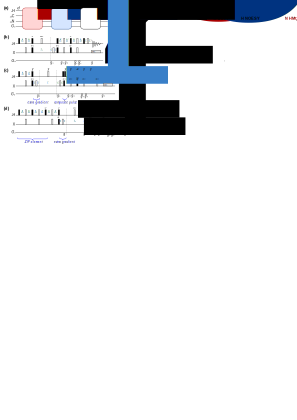
\includegraphics[width=0.6\textwidth]{pprogs.png}
    {\phantomsubcaption\label{fig:pprogs_overview}}
    {\phantomsubcaption\label{fig:pprogs_crk}}
    {\phantomsubcaption\label{fig:pprogs_spv1}}
    {\phantomsubcaption\label{fig:pprogs_spv2}}
    \caption{
        \textbf{\subref{fig:pprogs_overview}} Overview of a typical NOAH supersequence (MSCN, using the single-letter abbreviations previously defined\autocite{Kupce2017ACIE}).
        The \nitrogen{}--\proton{} HMQC and \carbon{}--\proton{} HSQC modules are coloured; these may be replaced with the new seHSQC module proposed in this work.
        \textbf{\subref{fig:pprogs_crk}} Cavanagh--Rance--Kay (CRK) seHSQC.\autocite{sehsqc}
        \textbf{\subref{fig:pprogs_spv1}} Version 1 of the NOAH seHSQC module, abbreviated as ``\noahSpa{}''.
        \textbf{\subref{fig:pprogs_spv2}} Version 2 of the NOAH seHSQC module, abbreviated as ``\noahSpb{}''.
        Filled and unfilled bars represent \ang{90} and \ang{180} pulses respectively; all \ang{180} pulses on \carbon{} are adiabatic (frequency-swept) pulses.
        All pulses are applied along $+x$ unless otherwise noted.
        Phase cycling is performed with $\phi_1 = (x, -x)$ and $\phi_2 = (x, x, -x, -x)$.
        The delays are chosen as follows: $\Delta = 1/(4\cdot\onejxh)$, $\Delta' = 1/(8\cdot\onejch)$ or $1/(4\cdot\onejnh)$, and $\varepsilon$ is the minimum time needed for a gradient pulse and subsequent recovery.
        All gradient pulses are \SI{1}{\ms} long, except for $g_1$ and $g_2$ in \nitrogen{} experiments which are \SI{2.5}{\ms} long.
        Gradient amplitudes, as percentages of maximum gradient strength, are as follows: $g_1 = 80\%$; $g_2 = \pm 40.2\%$ (\carbon{}) or $\pm 16.2\%$ (\nitrogen{}); ${g_2}' = g_2/2$; $g_3 = 11\%$; $g_4 = -5\%$.
        The signs of $g_2$ and ${g_2}'$, as well as the phase of the \ang{90} X pulse marked $\pm y$, are alternated within each $t_1$ increment to provide echo--antiecho selection.
        Refer to \cref{fig:pprogs_prodop} for product operator analysis.
    }
    \label{fig:pprogs}
\end{figure}

A typical example of a NOAH supersequence is the NOAH-4 MSCN experiment (\cref{fig:pprogs_overview}), which yields \nitrogen{} H\textbf{M}QC, \carbon{} H\textbf{S}QC, \textbf{C}OSY, and \textbf{N}OESY spectra in one single experiment.\autocite{Kupce2017ACIE}
The implementation of this supersequence relies on the fact that the output of any one module contains all the necessary magnetisation components required for downstream modules.
For example, both the standard NOAH HMQC (\cref{fig:pprogs_prodop_hmqc})\autocite{Kupce2017ACIE, Kupce2007MRC} and HSQC (\cref{fig:pprogs_prodop_hsqc})\autocite{Kupce2017ACIE, Schulze-Sunninghausen2017JMR} modules return the bulk \magnnot{\ce{X}} magnetisation back to its equilibrium position ($+z$).
In the MSCN sequence, this bulk magnetisation can therefore be used as the input to the COSY and NOESY homonuclear modules which follow.
However, the original Cavanagh--Rance--Kay (CRK) seHSQC (\cref{fig:pprogs_crk}) does not obey this principle: it causes bulk magnetisation to be dephased by coherence transfer pathway (CTP) gradients.
Consequently, downstream modules can only utilise any bulk \magnnot{\ce{X}} magnetisation that has relaxed during the HSQC FID acquisition, leading to drastic losses in signal intensity.
This is illustrated using a NOAH-2 \noahtwo{Sp}{Cc} (seHSQC + CLIP-COSY\autocite{Koos2016ACIE}) supersequence: the CLIP-COSY is used in this work as a convenient module for which peaks can be easily integrated, but the conclusions drawn here are fully applicable to any other homonuclear module that is used in its place.
While the CRK seHSQC implementation (\cref{fig:sehsqc_comp_crk}) affords significant sensitivity gains (primarily for CH peaks, as predicted by theory\autocite{sehsqc_sens}), the COSY module which follows suffers from an almost complete ($\sim 90\%$) loss of intensity.
While one could argue that this is still tolerable for the COSY module, which is the most sensitive of all NOAH modules, these losses are not permissible for less inherently sensitive homonuclear modules such as NOESY and ROESY.

\begin{figure}
    \centering
    % figures/sehsqc_comp.py
    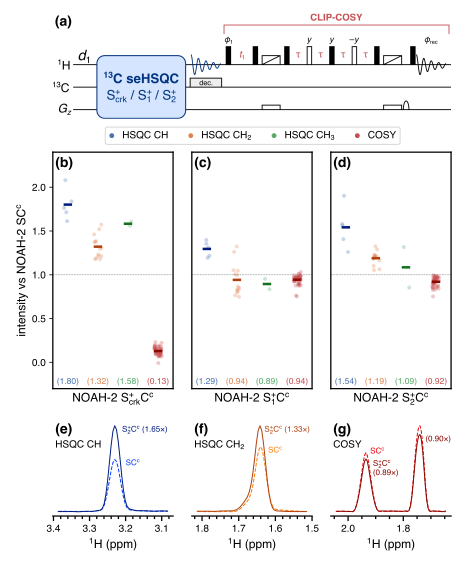
\includegraphics[width=0.6\textwidth]{sehsqc_comp.png}
    {\phantomsubcaption\label{fig:sehsqc_comp_crk}}
    {\phantomsubcaption\label{fig:sehsqc_comp_spv1}}
    {\phantomsubcaption\label{fig:sehsqc_comp_spv2}}
    {\phantomsubcaption\label{fig:sehsqc_comp_ex_ch}}
    {\phantomsubcaption\label{fig:sehsqc_comp_ex_ch2}}
    {\phantomsubcaption\label{fig:sehsqc_comp_ex_cosy}}
    \caption{
        Sensitivity comparisons for NOAH-2 \noahtwo{Sp}{Cc} (seHSQC + CLIP-COSY) supersequences, using the CRK and NOAH seHSQC implementations.
        The delay $\Delta'$ was set to $1/(8\cdot\onejch)$.
        All intensities are normalised against the NOAH-2 \noahtwo{S}{Cc} (HSQC + CLIP-COSY) supersequence, without HSQC sensitivity enhancement.
        HSQC intensities are further grouped by multiplicity.
        Circles represent the relative intensities of individual peaks; solid bars, as well as the numbers in parentheses, indicate averages over all peaks of a given type.
        \textbf{\subref{fig:sehsqc_comp_crk}} Using the original CRK seHSQC (\cref{fig:pprogs_crk}).
        The CRK seHSQC does not preserve the bulk \magnnot{\ce{X}} magnetisation, leading to severely reduced COSY intensities.
        \textbf{\subref{fig:sehsqc_comp_spv1}} Using the \noahSpa{} module (\cref{fig:pprogs_spv1}).
        \textbf{\subref{fig:sehsqc_comp_spv2}} Using the \noahSpb{} module (\cref{fig:pprogs_spv2}).
        \textbf{\subref{fig:sehsqc_comp_ex_ch}--\subref{fig:sehsqc_comp_ex_ch2}} Slices of the NOAH HSQC (dashed line) and NOAH ZIP-seHSQC (\noahSpb{}) spectra (solid line) through $f_1 = \SI{78.9}{\ppm}$ (a \ce{CH} peak, \subref{fig:sehsqc_comp_ex_ch}) and $f_1 = \SI{28.5}{\ppm}$ (a \ce{CH2} peak, \subref{fig:sehsqc_comp_ex_ch2}).
        \textbf{\subref{fig:sehsqc_comp_ex_cosy}} Slices of the CLIP-COSY module from the NOAH-2 \noahtwo{S}{Cc} (dashed line) and \noahtwo{Spb}{Cc} (solid line) supersequences, through $f_1 = \SI{1.36}{\ppm}$.
        \andro{}
    }
    \label{fig:sehsqc_comp}
\end{figure}

In this work, we compare two possible solutions to this, which form the basis of the NOAH seHSQC modules.
In both cases, we require a pulse sequence element which performs a selective \ang{90} rotation on \magn{\ce{X}} magnetisation and leaves \magnnot{\ce{X}} magnetisation untouched.
The first version of the NOAH seHSQC (\cref{fig:pprogs_spv1}, ``\noahSpa'') uses a composite \proton{} pulse immediately following $t_1$ to accomplish this aim, as both magnetisation components have already diverged by this point.
On the other hand, the second (\cref{fig:pprogs_spv2}, ``\noahSpa'' or ``ZIP-seHSQC'') actively differentiates the two components at the start of the sequence by prepending a double heteronuclear spin echo, a strategy recently reported by Hansen \textit{et al.}\autocite{Hansen2021}
This $zz$ isotope-selective (ZIP) pulse element is based on the observation that the bulk \magnnot{\ce{X}} magnetisation in the seHSQC will be returned to $+z$ if the phase of the initial \proton{} $90^\circ_{x}$ pulse in the CRK seHSQC is changed by \ang{90} to $+y$.
To generate the required HSQC signal, however, a \proton{} $90^\circ_x$ pulse must still be applied to \magn{\ce{X}} magnetisation.
Overall, what is required is therefore a pulse sequence element which simultaneously acts as a $90^\circ_x$ (or $90^\circ_{-x})$ pulse on protons coupled to spin-\ce{X}, and as a $90^\circ_y$ pulse on uncoupled protons.
The resulting ZIP element is similar to the $zz$-filter, which has previously been used in the NOAH $zz$-HMBC module to retain the magnetisation of directly coupled protons for a subsequent HSQC module.\autocite{Kupce2018CC, Kupce2019JMR}
However, the ZIP element has different pulse phases to this and consequently leads to a different overall outcome, i.e.\ $90^\circ_{-x}$ on \magn{\ce{X}} and $90^\circ_y$ on \magnnot{\ce{X}}.

In addition to the aforementioned modifications, both NOAH seHSQC modules also contain a CTP gradient prior to the $t_1$ period (highlighted in \cref{fig:pprogs_spv1,fig:pprogs_spv2}).
In the \noahSpa{} module, the \magnnot{\ce{X}} magnetisation is in the $xy$-plane during $t_1$ (see \cref{fig:pprogs_prodop} for product operator analysis), and would simply be dephased if this gradient were not present, making its presence mandatory.
Alternatively, the \noahSpb{} module places the \magnnot{\ce{X}} magnetisation on $\pm z$ in $t_1$.
This gradient is therefore not used for rephasing, but instead serves to suppress artefacts in downstream modules, which would otherwise arise from bulk magnetisation that (due to pulse imperfections) is \textit{not} longitudinal and can therefore evolve during either half of the HSQC $t_1$ period (\cref{fig:wing_artefacts,fig:wing_artefacts2,fig:wing_gradients}).
This magnetisation then evolves again in the $t_1$ period of a later homonuclear module (e.g.\ COSY), resulting in each COSY peak with indirect-dimension frequency $f_1 = \Omega_{\ce{H}}$ being accompanied by a pair of ``wing'' artefacts at $f_1 = \Omega_{\ce{H}} \pm (\Omega_{\ce{H}}\cdot\mathrm{SW_{COSY}})/(2\cdot \mathrm{SW_{HSQC}})$, where $\Omega_{\ce{H}}$ and SW refer to the proton offset and indirect-dimension spectral width respectively (both in Hz).
Importantly, the artefacts arising from diagonal peaks can have intensities that are comparable to genuine crosspeaks (\cref{fig:wing_artefacts}), which highlights the importance of suppressing these artefacts.
Apart from the ``wing'' artefacts in downstream modules, we also briefly note here that the presence of two CTP gradients inside the seHSQC $t_1$ period allows the final CTP gradient ($g_2$) to have twice its usual amplitude, thereby providing additional artefact suppression in the seHSQC itself.
This is particularly important in the \nitrogen{}--\proton{} seHSQC, as will be explained below.

Both NOAH seHSQC modules provide clear sensitivity gains over the NOAH HSQC module for CH peaks (\cref{fig:sehsqc_comp_spv1,fig:sehsqc_comp_spv2,fig:sehsqc_comp_ex_ch}), though for \ce{CH2} and \ce{CH3} peaks, when the delay $\Delta'$ is set to $1/(8 \cdot \onejch)$ as done here, the gains achieved via sensitivity enhancement are rather more modest (the case where $\Delta' = 1/(4\cdot\onejch)$ is explored in \cref{fig:1_4j_unedited}).\autocite{Schleucher1994JBNMR}
Furthermore, the modifications present in the NOAH seHSQC invariably make them less efficient as compared to the original CRK implementation.
Consequently, in this example, the use of the \noahSpa{} module does not provide any sensitivity enhancement for \ce{CH2} and \ce{CH3} peaks, whilst the \noahSpb{} module yields on average $1.19\times$ increased sensitivity for \ce{CH2} peaks (\cref{fig:sehsqc_comp_ex_ch2}).
The new seHSQC modules, however, bring about dramatic improvements in the homonuclear module which follows.
In contrast to the CRK seHSQC, which largely destroys the requisite bulk magnetisation, both seHSQC modules preserve the majority of it, performing $>$90\% as well as the original HSQC module (\cref{fig:sehsqc_comp_ex_cosy}).
We note that the BIG-BIRD element reported by Briand and S{\o}rensen\autocite{Briand1997JMR}, which independently excites \magn{\ce{X}} and \magnnot{\ce{X}} magnetisation with arbitrary flip angles and phases, is also capable of performing the same role as the ZIP element in the \noahSpb{} module.
However, we find that the ZIP provides greater signal-to-noise in both the seHSQC itself as well as downstream modules (\cref{fig:bigbird}).

Multiplicity editing\autocite{Parella1997JMR} can be easily incorporated into both NOAH seHSQC modules (\cref{fig:mult_edit}) by introducing a $J$-evolution period in the spin echo immediately following $t_1$.
As described previously, the \noahSpa{} module places the bulk magnetisation in the $xy$-plane during the editing period; the same is true of the unenhanced NOAH HSQC.
In these modules, the bulk \magnnot{\ce{X}} magnetisation is therefore subject to homonuclear coupling ($\jhh$) evolution, leading to a small decrease in the sensitivity of later homonuclear modules when multiplicity editing is introduced.
Since homonuclear experiments typically have a greater inherent sensitivity than the (se)HSQC, this minor loss is rarely a problem, and is far outweighed by the benefits of incorporating multiplicity editing in the HSQC.
Nevertheless, the fact that the \noahSpb{} module does not suffer from such a penalty is a welcome benefit.
As a result, when editing is included, the \noahSpb{} module slightly outperforms both the \noahS{} and \noahSpa{} modules by around 10\% in terms of preserving bulk magnetisation (\cref{fig:edited_sn_comp}).
% }}}
% 15N seHSQC {{{

The proposed seHSQC modules can be similarly implemented for \nitrogen{} experiments.
Currently, in NOAH supersequences, \nitrogen{}--\proton{} correlations are primarily obtained using the HMQC module;\autocite{Kupce2007MRC, Kupce2017ACIE} compared to this, the new \noahSpb{} module can provide greater than $4\times$ enhanced sensitivity (\cref{fig:15n_spv2vsm}).
This arises partly because the PEP sensitivity enhancement scheme can be optimised for \ce{NH} peaks by setting the reverse INEPT transfer delay $\Delta'$ to be equal to $1/(4 \cdot\onejnh)$.
However, there is also a significant improvement due to the fact that peaks in the \nitrogen{} seHSQC are not broadened in the indirect dimension by $\jhh$, unlike in the \nitrogen{} HMQC.
Although the \noahSpb{} module retains a slightly smaller amount of \magnnot{\ce{N}} magnetisation ($\sim 70\%$, versus $\sim 80\%$ for the HMQC (\cref{fig:n15_bulk_retention})), this is unlikely to be problematic, since it is the \nitrogen{} module which typically has the lowest intrinsic sensitivity in a supersequence.

\begin{figure}
    \centering
    % figures/15n_spv2vsm.py
    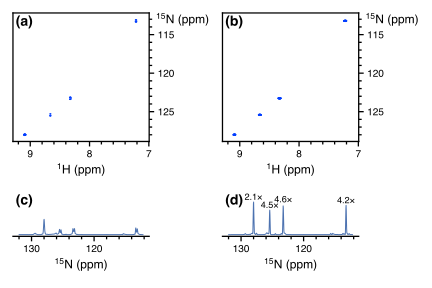
\includegraphics[width=0.6\textwidth]{15n_spv2vsm.png}
    {\phantomsubcaption\label{fig:15n_spv2vsm_hmqc}}
    {\phantomsubcaption\label{fig:15n_spv2vsm_spv2}}
    {\phantomsubcaption\label{fig:15n_spv2vsm_hmqc_proj}}
    {\phantomsubcaption\label{fig:15n_spv2vsm_spv2_proj}}
    \caption{
        Comparison of the \nitrogen{}--\proton{} seHSQC module (\noahSpb{}) with the standard NOAH HMQC module (\noahM{}), taken from NOAH-3 \noahthree{X}{Sp}{Cc} supersequences (\nitrogen{} experiment + \carbon{} seHSQC + CLIP-COSY).
        The \noahSpa{} module is not shown here as it causes line broadening downstream modules (see text).
        \textbf{\subref{fig:15n_spv2vsm_hmqc}} \nitrogen{} HMQC spectrum.
        \textbf{\subref{fig:15n_spv2vsm_spv2}} \nitrogen{} seHSQC spectrum.
        \textbf{\subref{fig:15n_spv2vsm_hmqc_proj}} Projection of HMQC onto the $f_1$ axis.
        Splitting due to $\jhh$ is clearly visible for three of the four peaks.
        \textbf{\subref{fig:15n_spv2vsm_spv2_proj}} Projection of seHSQC onto the $f_1$ axis.
        Signal-to-noise improvements relative to the HMQC spectrum are indicated over each peak.
        The largest gains are observed for peaks where the multiplet structure is collapsed; however, even in the absence of that, a $\sim 2\times$ gain is still obtained.
        \grami{}
    }
    \label{fig:15n_spv2vsm}
\end{figure}

Although the \noahS{} and \noahSpa{} modules also provide sensitivity gains versus the HMQC, they both come with other drawbacks.
As previously discussed, these two modules place bulk \magnnot{\ce{N}} magnetisation in the $xy$-plane during the $t_1$ period.
Consequently, the amount of bulk magnetisation that is retained decreases as $t_1$ is lengthened, leading to line broadening in the indirect dimensions of all downstream modules (\cref{fig:n15_linebroadening}).
Whilst this is not a problem with the \carbon{} HSQC where typical \carbon{} indirect dimension acquisition times are relatively short, the smaller spectral widths in \nitrogen{} experiments can mean downstream modules suffer moderate losses in both sensitivity and resolution.
The \noahSpb{} module avoids this issue entirely, making it especially well-suited to obtaining \nitrogen{} correlations; we henceforth refer to it as the \noahSpn{} module.

One remaining potential issue in the \noahSpn{} module arises from the cumulative effects of pulse imperfections, which cause a portion of bulk \magnnot{\ce{N}} magnetisation to be transverse just prior to detection of the seHSQC signal.
Although this only represents a small fraction of the bulk magnetisation, if left uncontrolled, the resulting artefacts typically have intensities that are comparable to the seHSQC crosspeaks (\cref{fig:cnst16_diff}).
The key to suppressing these artefacts efficiently lies in the final CTP gradient $g_2$ (\cref{fig:pprogs_spv2}), which dephases any transverse bulk magnetisation.
The \noahSpn{} module therefore greatly benefits from having two CTP gradients $g_1$ within the $t_1$ period, as this means that $g_2$ will have twice its usual amplitude.
For optimal performance, however, one further modification proves beneficial: the CTP gradients $g_1$ and $g_2$ should all be lengthened from their typical duration of \SI{1}{\ms}, in order to provide more effective dephasing.
In practice, we find that gradient durations of 2 to \SI{2.5}{\ms} provide excellent artefact suppression whilst not causing any appreciable difference in the intensity of the desired crosspeaks (\cref{fig:cnst16_diff}).
These extended gradients are not required in the \carbon{} seHSQC for two reasons: firstly, the amplitude of $g_2$ in the \carbon{} seHSQC is larger by a factor of $\gamma_{\ce{C}}/\gamma_{\ce{N}} \approx 2.5$; and secondly, the greater natural abundance of \carbon{} (1.1\% versus 0.36\% of \nitrogen{}) leads to an intrinsically larger signal intensity, which makes any residual artefacts less apparent.

In scenarios where high resolution in the \nitrogen{} dimension is not required, it can prove useful to reduce the number of $t_1$ increments and in its place increase the number of transients acquired.\autocite{Perez-Trujillo2007MRC, Parella2010CMR}
In new versions of the NOAH pulse programmes (including those provided in the \SInf{}), this feature can be enabled by specifying a factor $k$ by which to perform this scaling.
Note that the scaling is only applied to the \nitrogen{} module; all other modules are left untouched.
In our hands, setting $k = 2$ or 4 for the original \nitrogen{} HMQC can lead to significant sensitivity gains of up to $\sim 2\times$, since $\jhh$ splitting in the indirect dimension tends not to be resolved (\cref{fig:hmqc_kscale}).
This point is not relevant to the seHSQC, and here $k$-scaling employed in isolation has only a tiny effect on peak height (and signal-to-noise), since any sensitivity gained from the extra transients is typically offset by the broadening (\cref{fig:spv2_kscale}).
However, the later $t_1$ increments which were not acquired can be reconstructed using linear projection\autocite{linearpred} to mitigate this line broadening.
The resulting spectra display sensitivity gains of up to a factor of $k$, although the fidelity of the reconstruction can suffer for large $k$, particularly with the HMQC (\cref{fig:hmqc_kscale_lp,fig:spv2_kscale_lp}).

% }}}
% Double HSQC and HSQC-TOCSY {{{

\begin{figure}
    \centering
    % Inkscape
    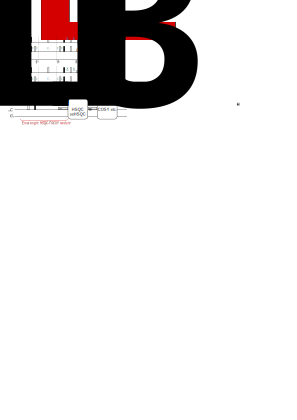
\includegraphics[width=0.7\textwidth]{pprogs_hsqct.png}
    {\phantomsubcaption\label{fig:pprogs_hsqct_hsqc}}
    {\phantomsubcaption\label{fig:pprogs_hsqct_hsqct}}
    {\phantomsubcaption\label{fig:pprogs_hsqct_superseq}}
    \caption{
        \textbf{\subref{fig:pprogs_hsqct_hsqc}} NOAH HSQC module with modified INEPT delay $\Delta_{\mathrm{E}} = (\sin^{-1} f)/(4\cdot\onejch)$, where $f$ is the fraction of \magn{\ce{C}} magnetisation excited.
        \textbf{\subref{fig:pprogs_hsqct_hsqct}} NOAH HSQC-TOCSY module (``\noahSt{}''), modified from the ASAP-HSQC-TOCSY.\autocite{Becker2019JMR}
        The gradients $g_3$ are \SI{1}{\ms} long, and are set to 19\% of the maximum gradient amplitude.
        \textbf{\subref{fig:pprogs_hsqct_superseq}} Overview of a NOAH-3 \noahthree{St}{S}{X} or \noahthree{St}{Sp}{X} supersequence.
        The \magn{\ce{C}} magnetisation is partly used by the initial HSQC-TOCSY module, with a subsequent HSQC or seHSQC using the remaining \magn{\ce{C}} magnetisation.
        The bulk \magnnot{\ce{C}} magnetisation is retained for one or more homonuclear modules at the end.
        All other symbols have the same meanings as in \cref{fig:pprogs}.
    }
    \label{fig:pprogs_hsqct}
\end{figure}

Next, we note that the HSQC module (though not the new seHSQC modules) allows an arbitrary amount of \magn{\ce{C}} magnetisation to be excited, with the remainder returned to $+z$.\autocite{Kupce2007MRC, Schulze-Sunninghausen2014JACS, Schulze-Sunninghausen2017JMR, Koos2019JMR}
In order to excite a proportion $f$ of \magn{\ce{C}} magnetisation ($0 < f \leq 1$), the initial INEPT delay must be shortened by a factor of $\sin^{-1}f$ (\cref{fig:pprogs_hsqct_hsqc}).
The remaining $(1 - f)$ of the magnetisation, plus any that relaxes during the HSQC FID, can then be used for a \textit{second} HSQC-based module in the same supersequence.
Such a scheme proves to be useful for simultaneously collecting \carbon{}-decoupled and coupled HSQC spectra, or HSQC spectra with different spectral widths.
This has previously been accomplished in a multi-FID acquisition (MFA) scheme by keeping the two CTPs in the CRK seHSQC separate, with the cosine- and sine-modulated CTPs each contributing to one spectrum.\autocite{ctphsqc}
With the present NOAH strategy, for values of $f$ that are close to 1, the amount of \magn{\ce{C}} magnetisation regained through relaxation can reach almost 50\%.
Consequently, by setting $f \approx 0.8$, we can obtain two HSQC spectra with sensitivities that are comparable to the existing MFA approach.
Furthermore, the sensitivity of the second HSQC can be boosted by using the new seHSQC modules in its place, in particular the \noahSpb{} module (\cref{fig:ssc_comparisons}).

By adding a period of isotropic mixing prior to detection, the NOAH HSQC module may be converted to a HSQC-TOCSY module (denoted by ``\noahSt{}'', \cref{fig:pprogs_hsqct_hsqct}).
This is similar to the previously reported ASAP-HSQC-TOCSY,\autocite{Becker2019JMR} the key difference being that in the present NOAH context, unused \magn{\ce{C}} as well as bulk \magnnot{\ce{C}} magnetisation is preserved for use in other modules, instead of later $t_1$ increments as in the ASAP experiment.
Compared to the existing MFA HSQC-TOCSY/HSQC experiment,\autocite{Nolis2019CPC} our approach has several characteristics which make it particularly amenable to use in NOAH supersequences.
Firstly, the vast majority of \magnnot{\ce{C}} magnetisation is preserved, as required for homonuclear module(s) to be appended in a NOAH supersequence (\cref{fig:pprogs_hsqct_superseq}); in practice, we observe small \magnnot{\ce{C}} losses of ca.\ 10\% due to pulse imperfections.
In contrast, the MFA sequence, much like the original CRK seHSQC on which it is based, dephases \magnnot{\ce{C}} magnetisation and causes a 80--90\% sensitivity loss in downstream spectra.
Secondly, since each NOAH module is independently executed, the NOAH approach allows multiplicity editing to be selectively enabled for only the HSQC and not the HSQC-TOCSY, where accidental overlap may lead to crosspeaks being lost unexpectedly.
Lastly, the sensitivity of both spectra in a NOAH experiment can be optimised through the value of $f$; this allows a larger amount of \magn{\ce{C}} magnetisation to be used for the inherently less sensitive HSQC-TOCSY.
In our experience, setting $f = 0.9$ provides a good balance for \noahtwo{St}{S} combinations: the sensitivity in the HSQC is boosted not only by relaxation during the HSQC-TOCSY FID, but also by the isotropic mixing in the HSQC-TOCSY module, which effects a degree of \magnnot{\ce{C}}\,$\to\,$\magn{\ce{C}} polarisation transfer (\cref{fig:stsc_comparisons}).
Alternatively, the signal intensity of the HSQC-TOCSY can be maximised by replacing it with the seHSQC-TOCSY module, derived from the \noahSpb{} module.\autocite{Hansen2021}
The sole drawback of the seHSQC-TOCSY is that it does not allow for variable \magn{\ce{C}} excitation and therefore cannot preserve any magnetisation for HSQC modules that follow it (\cref{fig:sehsqc_tocsy}).

% }}}
% Example spectra {{{

\begin{figure}
    \centering
    % figures/spnstspcc.py
    \includegraphics[width=0.6\textwidth]{spnstspcc.png}
    {\phantomsubcaption\label{fig:spnstspcc_spn}}
    {\phantomsubcaption\label{fig:spnstspcc_st}}
    {\phantomsubcaption\label{fig:spnstspcc_sp}}
    {\phantomsubcaption\label{fig:spnstspcc_cc}}
    \caption{
        Spectra obtained from the NOAH-4 \noahfour{Spn}{St}{Spb}{Cc} supersequence.
        256 $t_1$ increments were used, with 2 scans per increment.
        The total experiment time was 17 minutes and 35 seconds.
        \textbf{\subref{fig:spnstspcc_spn}} \nitrogen{} seHSQC.
        \textbf{\subref{fig:spnstspcc_st}} \carbon{} HSQC-TOCSY (\SI{30}{ms} mixing, $f = 0.9$).
        \textbf{\subref{fig:spnstspcc_sp}} Multiplicity-edited \carbon{} ZIP-seHSQC. Notice that having the edited seHSQC removes the need for the less desirable HSQC-TOCSY editing.
        \textbf{\subref{fig:spnstspcc_cc}} CLIP-COSY.
        Spectra were obtained on a \SI{700}{\MHz} Bruker AV III equipped with a TCI H/C/N cryoprobe; the sample used was \SI{40}{\milli\molar} gramicidin (a cyclic decapeptide; \ce{(Val-Orn-Leu-$\text{{\scriptsize D}-}$Phe-Pro)2}) in DMSO-$d_6$.
    }
    \label{fig:spnstspcc}
\end{figure}

There exist many ways in which the new modules discussed above can be included in practical experiments for structure characterisation.
Here, we illustrate this with the NOAH-4 \noahfour{Spn}{St}{Spb}{Cc} (\nitrogen{} seHSQC, \carbon{} HSQC-TOCSY, \carbon{} seHSQC, and CLIP-COSY) supersequence (\cref{fig:spnstspcc}).
While individual collection of the four spectra above required 57 minutes and 8 seconds, the NOAH-4 supersequence took only 17 minutes and 35 seconds; this is $30.8\%$ of the original duration, or equivalently a $3.25\times$ speedup.
For typical organic molecules, new supersequences such as the NOAH-4 \noahfour{St}{Spb}{C}{T} allow the rapid and complete collection of \ce{C-H} and \ce{H-H} correlations (\cref{fig:stspct}).
Experiment times can be further reduced through the use of non-uniform sampling\autocite{nus} (\cref{fig:stspct_nus}), which is compatible with nearly all of the supersequences shown here (the only exceptions being when $k$-scaling is employed in \nitrogen{} modules, or when COSY modules are recorded without phase-sensitive detection).
One can also prepend the NOAH $zz$-HMBC module (``\noahB{}'');\autocite{Kupce2019JMR} this uses the semi-adiabatic $zz$-filter to preserve both \magn{\ce{C}} and \magn{\ce{N}} magnetisation, which can then be sampled in the HSQC-based modules presented here (\cref{fig:bspnspcqf}).

% }}}
% {{{ Benefits of time savings incl. sensitivity
The benefits of the time savings afforded by NOAH supersequences are manifold.
Apart from the enabling of greatly increased sample throughput, the combination of multiple modules in a single experiment also ensures that all constituent spectra are recorded under the same experimental conditions, such as temperature.
This avoids the need for separate chemical shift referencing in each spectrum, and also makes the real-time monitoring and characterisation of reactive intermediates possible, especially when combined with non-uniform sampling.
It is also of note that time savings may be directly translated into increases in sensitivity per unit time.
The \textit{relative sensitivity per unit time}, $\varepsilon_t$, of a given module is the product of an \textit{amplitude factor} $R_S$ indicating the intrinsic sensitivity of a module with respect to a reference experiment, and the square root of a \textit{time-saving factor} $\rho_t$, which reflects the decrease in time needed for collection of all spectra.

We demonstrate this with the NOAH-4 \noahfour{Spn}{Spb}{C}{T} supersequence (experimental time of 17 minutes and 28 seconds), choosing individually acquired versions of the four constituent modules as the reference spectra (total experimental time of 58 minutes and 42 seconds), which gives $\rho_t = 3.36$.
The amplitude factor $R_S$ starts off at 1 for the first module, with a slight decrease as the supersequence progresses due to imperfections in magnetisation preservation.
Nevertheless, $\varepsilon_t$ remains well above 1 for all four modules (\cref{fig:snr_modules}), which clearly illustrates the attainable gains in sensitivity per unit time in NOAH sequences where $R_S$ is not significantly compromised: this is especially important for the heteronuclear modules which are naturally less sensitive.
Comparisons against ``standard'' experiments (such as the CRK seHSQC) lead to similar conclusions (\cref{fig:snr_bruker}).

\begin{figure}
    \centering
    % figures/snr_modules.py
    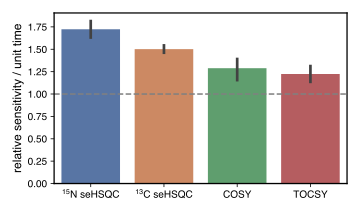
\includegraphics[width=0.6\textwidth]{snr_modules.png}
    \caption{
        Relative sensitivities per unit time ($\varepsilon_t$) for the four modules in the \noahfour{Spn}{Spb}{C}{T} supersequence (using a TOCSY mixing time of \SI{35}{\ms}).
        Error bars indicate 95\% confidence intervals.
        The four NOAH modules, individually acquired, were used as the reference spectra ($\rho_t = 3.36$).
        \zolmi{}
    }
    \label{fig:snr_modules}
\end{figure}

% }}}
% Conclusion {{{

The new seHSQC and HSQC-TOCSY implementations add to the preexisting variety of NOAH modules, expanding the number of plausible NOAH supersequences tailored for small molecule characterisation.
The controlled manipulation of all proton magnetisation reservoirs present within a sample is required for the success of these modules within nested experiments.
We have demonstrated the optimisation of the individual HSQC-based modules and their combinations to further enhance the diversity of NOAH supersequences for efficient data collection.
% }}}
% Experimental {{{

\textbf{\Large Experimental}

All spectra were recorded on a Bruker AV III NMR spectrometer operating at \SI{700}{\MHz} \proton{} frequency equipped with a TCI H/C/N cryoprobe.
Unless otherwise specified, spectra were recorded with 16 dummy scans, 2 scans per $t_1$ increment, 256 $t_1$ increments per module, and a \SI{1.5}{\s} recovery delay.
1024 points were recorded in each FID, leading to an acquisition time of 60.8--\SI{73.1}{\ms} depending on the \proton{} spectral width (10--\SI{12}{\ppm}).
The delays in the HSQC sequences were optimised for $\onejch = \SI{145}{\Hz}$ and $\onejnh = \SI{90}{\Hz}$ respectively, and the CLIP-COSY mixing delay (denoted by $\Delta$ in the original work\autocite{Koos2016ACIE}) was set to \SI{16.7}{\ms} (corresponding to a nominal $\jhh$ value of \SI{30}{Hz}).
DIPSI-2 mixing in the HSQC-TOCSY was applied with a $B_1$ amplitude of \SI{10}{\kHz}.


All NOAH data were processed using the \texttt{splitx\_au} AU programme, available in the standard Bruker TopSpin software, which separates the individual modules into different datasets; these were then individually processed with \texttt{noah\_EXPT} AU programmes, which define other processing parameters such as window functions.
All datasets were linear predicted up to 512 complex points in $f_1$, then zero-filled to 1024 and 2048 complex points in $f_1$ and $f_2$ respectively.
NUS experiments, such as that in \cref{fig:stspct_nus}, can be set up using a new \texttt{noah\_nus2.py} Python script.
The pulse sequences used here, all AU processing scripts, as well as the NUS Python script are available from the authors upon request, and will also be made available via the online Bruker User Library.

% }}}
% Acknowledgements {{{

\textbf{\Large Acknowledgements}

J.R.J.Y.\ thanks the Clarendon Fund (University of Oxford) and the EPSRC Centre for Doctoral Training in Synthesis for Biology and Medicine (EP/L015838/1) for a studentship, generously supported by AstraZeneca, Diamond Light Source, Defence Science and Technology Laboratory, Evotec, GlaxoSmithKline, Janssen, Novartis, Pfizer, Syngenta, Takeda, UCB, and Vertex.
Helpful discussions\ldots
Other acknowledgements\ldots

% }}}
% Bibliography and SI {{{
\printbibliography
\end{refsection}
\begin{refsection}
% Fakesection Preamble-ish commands
\newcommand{\sectionbreak}{\clearpage}
\renewcommand\thefigure{S\arabic{figure}}
\renewcommand\thetable{S\arabic{table}}
\setcounter{page}{1}
\setcounter{figure}{0}
\setcounter{table}{0}
\onehalfspacing

% Fakesection Title page
\hspace{0pt}
\vfill
\begin{center}
    \huge
    Supporting Information

    \textit{for}

    Diversifying NOAH Supersequences with New HSQC-based Modules

    \vspace{1cm}

    \Large Jonathan R. J. Yong,\textsuperscript{1} {\=E}riks Kup{\v{c}}e,\textsuperscript{2} Tim D. W. Claridge\textsuperscript{1,}*

    \vspace{1cm}

    \large \textsuperscript{1} \textit{Chemistry Research Laboratory, Department of Chemistry, University of Oxford, Mansfield Road, Oxford, OX1 3TA, U.K.}

    \textsuperscript{2} \textit{Bruker UK Ltd., Banner Lane, Coventry, CV4 9GH, U.K.}

    * \texttt{tim.claridge@chem.ox.ac.uk}
\end{center}
\thispagestyle{empty}
\vfill
\hspace{0pt}
\newpage

% Fakesection Table of contents
\tableofcontents

\newpage

\section{Product operator analysis}

... 

\section{Multiplicity editing in seHSQC}

\begin{figure}
    \centering
    % done in Inkscape
    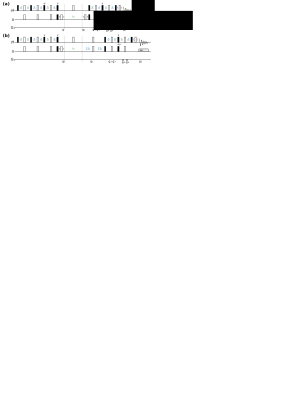
\includegraphics[width=0.8\textwidth]{./figures/mult_edit.png}
    \caption{
        Implementation of multiplicity editing in the new NOAH seHSQC module.
        \textbf{(a)} Unedited NOAH seHSQC, as presented in the main text.
        \textbf{(b)} Edited NOAH seHSQC (note the different phase in the third \proton{} \ang{90} pulse; this is needed to compensate for the extra \ang{180} in the editing period).
        Symbols have the same meaning as in \figref{pprogs} of the main text.
    }
    \label{fig:edited_sehsqc_pprog}
\end{figure}

\begin{figure}
    \centering
    % figures/edited_sn_comp.py
    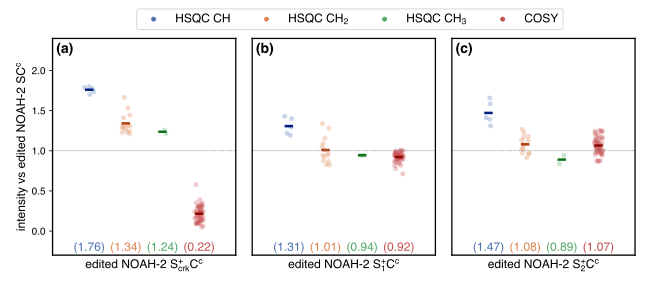
\includegraphics[width=0.8\textwidth]{./figures/edited_sn_comp.png}
    \caption{
        Sensitivity of edited seHSQC versus the NOAH HSQC/CLIP-COSY supersequence.
        \andro{}
        \textbf{(a)} CRK edited seHSQC + CLIP-COSY.
        Although larger gains are observed in the HSQC, the COSY intensities are severely decreased.
        \textbf{(b)} NOAH edited seHSQC + CLIP-COSY.
        On average, sensitivity gains are observed in both the HSQC and COSY modules (except for HSQC \ce{CH3} peaks).
    }
    \label{fig:edited_sn_comp}
\end{figure}

\section{Effect of setting \texorpdfstring{$\Delta' = 1/(4\cdot\onejch)$}{Delta' = 1/(4*1JCH)} in seHSQC}

The $\Delta'$ delay in the CRK and NOAH seHSQC sequences can be set to $1/(4\cdot\onejch)$ in order to optimise the sensitivity enhancement for \ce{CH} groups only.
The effects of doing so are shown here for the unedited and edited seHSQCs respectively.

\begin{figure}
    \centering
    % figures/combined_1_4j.py
    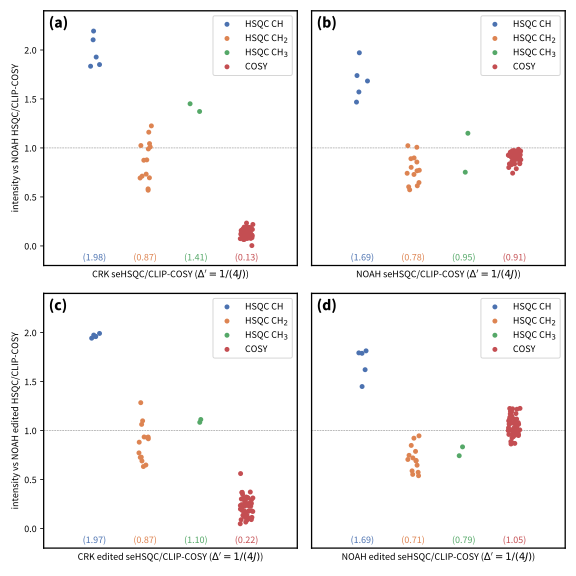
\includegraphics[width=0.8\textwidth]{./figures/combined_1_4j.png}
    \caption{
        Sensitivity of seHSQC sequences with $\Delta'$ set to $1/(4\cdot\onejch)$, versus the corresponding NOAH HSQC/CLIP-COSY supersequence (i.e.\ unedited for (a) and (b), edited for (c) and (d)).
        \andro{}
        \textbf{(a)} CRK seHSQC + CLIP-COSY, without multiplicity editing.
        \textbf{(b)} NOAH seHSQC + CLIP-COSY, without multiplicity editing.
        \textbf{(c)} CRK seHSQC + CLIP-COSY, with multiplicity editing.
        \textbf{(d)} NOAH seHSQC + CLIP-COSY, with multiplicity editing.
    }
    \label{fig:combined_1_4j}
\end{figure}

In particular, for the NOAH seHSQC, we note that the improvements in HSQC \ce{CH} sensitivity gained by moving from $\Delta' = 1/(8\cdot\onejch)$ to $\Delta' = 1/(4\cdot\onejch)$ are marginal (ca.\ 10\%).
At the same time, sensitivity \textit{losses} are observed for \ce{CH2} and \ce{CH3} peaks, likely due to pulse imperfections.

\section{Comparison of BIG-BIRD and ISR elements}

The BIG-BIRD element used here was ${45^\circ}_{45^\circ}(\proton{}) - 2\Delta - 180^\circ(\proton{},\carbon{}) - 2\Delta - {45^\circ}_{225^\circ}(\proton{})$ for the unedited NOAH seHSQC, where $\beta_\phi$ indicates a hard pulse with flip angle $\beta$ and phase $\phi$, and $\Delta = 1/(4\cdot\onejch)$.
For the edited NOAH seHSQC, the BIG-BIRD pulse phases are slightly modified to give ${45^\circ}_{315^\circ}(\proton{}) - 2\Delta - 180^\circ(\proton{},\carbon{}) - 2\Delta - {45^\circ}_{135^\circ}(\proton{})$.
These, and the ISR, have the same net effect on coupled and uncoupled proton magnetisation.
However, the ISR provides greater sensitivity in both the HSQC and downstream COSY.

\begin{figure}
    \centering
    % figures/bigbird.py
    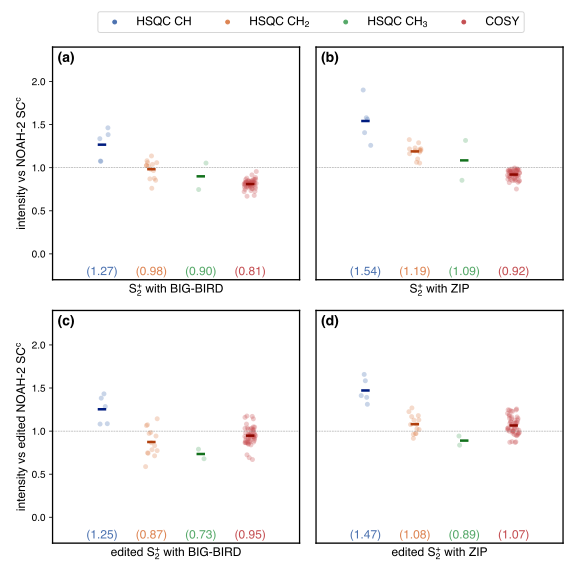
\includegraphics[width=0.8\textwidth]{./figures/bigbird.png}
    \caption{
        Sensitivity of NOAH seHSQC sequences with prepended BIG-BIRD and ISR elements, versus the corresponding NOAH HSQC/CLIP-COSY supersequence (i.e.\ unedited for (a) and (b), edited for (c) and (d)).
        \andro{}
        \textbf{(a)} NOAH seHSQC with BIG-BIRD + CLIP-COSY, without multiplicity editing.
        \textbf{(b)} NOAH seHSQC with ISR + CLIP-COSY, without multiplicity editing.
        \textbf{(c)} NOAH seHSQC with BIG-BIRD + CLIP-COSY, with multiplicity editing.
        \textbf{(d)} NOAH seHSQC with ISR + CLIP-COSY, with multiplicity editing.
    }
    \label{fig:bigbird}
\end{figure}


\section{Suppression of wing artefacts}

The origin of the ``wing'' artefacts in the final homonuclear modules can be most clearly seen from the following series of experiments involving the NOAH-3 \nitrogen{} seHSQC/\carbon{} seHSQC/CLIP-COSY (SpSpCc) supersequence.
Since the $f_1$ spectral windows of the two seHSQC modules are different, they lead to distinct sets of wing artefacts if the extra gradient before $t_1$ is not present.
\figref{wing_artefacts} focuses on the artefacts associated with intense methyl group peaks, but similar artefacts are observed for all other peaks, albeit with lower absolute intensities.

\begin{figure}
    \centering
    % figures/wing_artefacts.py
    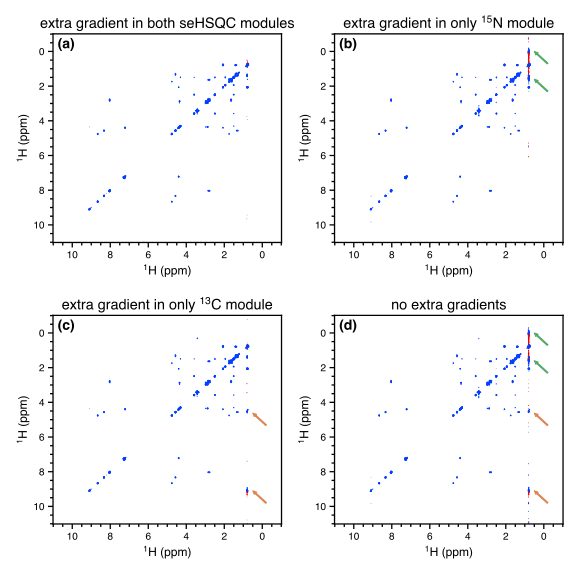
\includegraphics[width=0.8\textwidth]{./figures/wing_artefacts.png}
    \caption{
        CLIP-COSY spectra obtained from various forms of the NOAH-3 SpSpCc supersequence.
        Wing artefacts arising from the \nitrogen{} seHSQC are highlighted in orange; those arising from the \carbon{} seHSQC in green.
        Notice how (in this case) the former can easily be misinterpreted as a crosspeak, while the latter obscures genuine crosspeaks.
        \grami{}
        \textbf{(a)} With the extra gradient inserted for both modules, i.e.\ no artefacts.
        \textbf{(b)} With an extra gradient in only the \nitrogen{} module, i.e.\ only the \carbon{} artefacts.
        \textbf{(c)} With an extra gradient in only the \carbon{} module.
        \textbf{(d)} With no extra gradients.
    }
    \label{fig:wing_artefacts}
\end{figure}


\section{\texorpdfstring{\nitrogen{}}{15N} HSQC and line broadening}

For \nitrogen{}--\proton{} correlations, both the HMQC and the new seHSQC module are recommended as they keep the bulk magnetisation along $\pm z$ during the $t_1$ period.
The HSQC module places bulk magnetisation in the $xy$-plane, leading to $\jhh$ evolution; consequently, the amount of bulk magnetisation ``passed on'' to the downstream modules decreases as the \nitrogen{} $t_1$ is increased.
Since $t_1$ for each NOAH module is incremented in sync, this is manifested in downstream modules as a $t_1$-dependent decrease in amplitude, or $f_1$ line broadening after Fourier transformation, as shown in \figref{n15_linebroadening}.

\begin{figure}
    \centering
    % figures/n15_linebroadening.py
    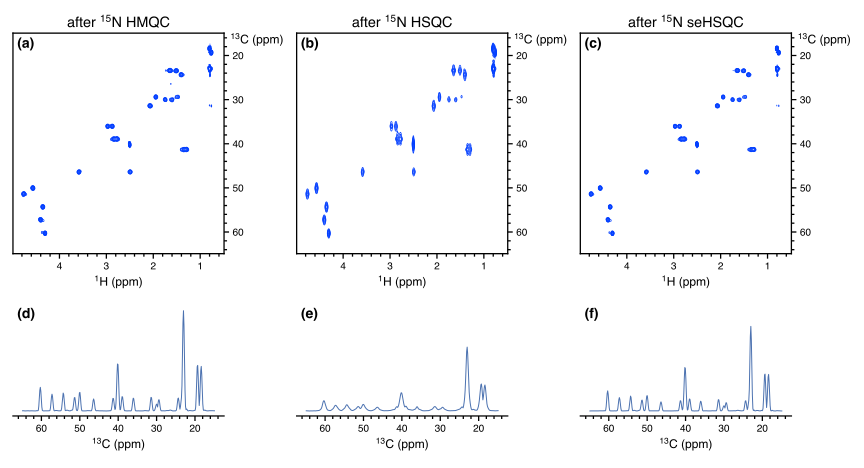
\includegraphics[width=\textwidth]{./figures/n15_linebroadening.png}
    \caption{
        \carbon{} seHSQC spectra obtained from NOAH-3 XSpCc (\nitrogen{} module + \carbon{} seHSQC + CLIP-COSY) supersequences.
        \grami{}
        The \nitrogen{} spectral window was \SI{30}{ppm} and 256 $t_1$ increments were collected, corresponding to an indirect-dimension \nitrogen{} acquisition time of \SI{60.1}{\ms}.
        \textbf{(a)} X = HMQC.
        \textbf{(b)} X = HSQC.
        \textbf{(c)} X = seHSQC.
        \textbf{(d)}--\textbf{(f)} Projections of spectra \textbf{(a)}--\textbf{(c)} onto the $f_1$ axis.
        Note the $f_1$ line broadening in (b) and (e).
    }
    \label{fig:n15_linebroadening}
\end{figure}

This line broadening also leads to a substantial sensitivity loss (almost 65\% in \figref{n15_linebroadening}).
The extent of the line broadening depends on the acquisition time, and is particularly pronounced for long acquisition times, i.e.\ small \nitrogen{} spectral windows.
In our experience, at \nitrogen{} acquisition times of ca.\ \SI{5}{\ms} the effect is almost indiscernible.
Such a short acquisition time would lead to poor resolution in the \nitrogen{} dimension itself, which may or may not be tolerable.
Of course, this issue can be entirely avoided by using either the HMQC or seHSQC.

\section{Effect of lengthened gradients in \texorpdfstring{\nitrogen{}}{15N} experiments}

cnst16 scan

\section{Effect of \texorpdfstring{$k$}{k}-scaling}

... both signal and artefact intensity, plus example spectra

\section{HSQC-TOCSY SNR comparisons}

... including Parella work

\section{Other example spectra}

...

\section{Pulse programmes}

...

\section{Processing scripts}

...

\end{refsection}
%}}}

\end{document}
